%%%%%%%%%%%%%%%%%%%%%%%%%%%%%%%%%%%%%%%%%%%%%%%%%%%%%%%%%%%%%%%%%%%
%   	FILL OUT METADATA IN PREAMBLE TEX FILE FIRST
%%%%%%%%%%%%%%%%%%%%%%%%%%%%%%%%%%%%%%%%%%%%%%%%%%%%%%%%%%%%%%%%%%%%
%%%%%%%%%%%%%%%%%%%%%%%%%%%%%%%%%%%%%%%%%%%%%%%%%%%%%%%%%%%%%%%%%%%
%     LaTeX source code to approximate a NIST Technical report
%	DOI and CrossMark watermark will be added on final PDF
% 	Developed by K. Miller, kmm5@nist.gov
%	Last updated: 21-June-2022
%%%%%%%%%%%%%%%%%%%%%%%%%%%%%%%%%%%%%%%%%%%%%%%%%%%%%%%%%%%%%%%%%%%
%%%%%%%%%%%%%%%%%%%%%%%%%%%%%%%%%%%%%%%%%%%%%%%%%%%%%%%%%%%%%%%%%%%
% Document class and template package DO NOT DELETE
%%%%%%%%%%%%%%%%%%%%%%%%%%%%%%%%%%%%%%%%%%%%%%%%%%%%%%%%%%%%%%%%%%%
\documentclass[12pt]{article}

\usepackage{settings}

%%%%%%%%%%%%%%%%%%%%%%%%%%%%%%%%%%%%%%%%%%%%%%%%%%%%%%%%%%%%%%%%%%%%%%%
% Publication Metadata
%%%%%%%%%%%%%%%%%%%%%%%%%%%%%%%%%%%%%%%%%%%%%%%%%%%%%%%%%%%%%%%%%%%%%%%
\newcommand{\pubseries}{Technical Note}
\newcommand{\pubnumber}{NIST TN 26xx}
\newcommand{\DOI}{https://doi.org/10.6028/NIST.TN.26xx}
\newcommand{\pubmonth}{December}
\newcommand{\pubyear}{2026}
%\newcommand{\erratadate}{03-14-2027}
\newcommand{\pubtitle}{Cable Aging Tests to assess fire performance of new and legacy cables (CAT-Fire)}
\newcommand{\pubsubtitle}{} % delete if no subtitle %
\newcommand{\draftstage}{Draft Stage} 
% Draft Stage is REQUIRED for drafts/preprints; Draft stages are listed in the NIST Publication Identifier guidance: https://www.nist.gov/nist-research-library/nist-technical-series-publications-author-instructions#pubid   %
\newcommand{\authorlist}{K. McGrattan; I. Leventon; Hamburger, K.;  Lee, A.}
\newcommand{\authorone}{Kevin McGrattan}
\newcommand{\authortwo}{Isaac Leventon}
\newcommand{\authorthree}{Kenneth Hamburger}
\newcommand{\authorfour}{Adam Lee}

\newcommand{\pubabstract}{This report documents a series of cable aging tests and related fire experiments conducted on coated and uncoated cables (thermoplastic and thermoset) representative of those typically found in nuclear power plants. The first object of these tests is to quantify the flammability response and potential for circuit failure of cables subjected to fire-like environments (i.e., radiant heating and direct flame impingment) when new and after accelerated aging protocols. The second objective of this report is to calibrate scaling parameters that enable prediction of expected cable performance after long-term use under ambient temperatures. 
	
	within steel electrical enclosures and on open ``ladder back'' cable trays. The first objective is to measure the heat release rates and qualitatively understand the burning behavior of circuit breaker fires within closed steel enclosures when ignited by a source representative of a high energy arc fault (HEAF). The second objective of this report is to quantify the thermal exposure of electrical cables that typically are installed in trays above an enclosure.  }
\newcommand{\keywords}{Aging; Cable Coatings; Cable Fires; Electrical fires}
\newcommand{\publang}{English} %If translation, change to correct language%
\usepackage{pdfproperties} 

\usepackage{multirow}  % Table formatting
\usepackage{placeins}  % FloatBarrier
\usepackage{subcaption} % Required package
\usepackage{graphicx}
%\usepackage[tagged,highstructure]{accessibility}

%%%%%%%%%%%%%%%%%%%%%%%%%%%%%%%%%%%%%%%%%%%%%%%%%%%%%%%%%%%%%%%%%%%%
%   	BEGIN DOCUMENT
%%%%%%%%%%%%%%%%%%%%%%%%%%%%%%%%%%%%%%%%%%%%%%%%%%%%%%%%%%%%%%%%%%%%
\begin{document}
	\urlstyle{rm} % Format style of \url
	% \linenumbers % Include if draft
	%%%%%%%%%%%%%%%%%%%%%%%%%%%%%%%%%%%%%%%%%%%%%%%%%%%%%%%%%%%%%%%%%%%%
	%   	DELETE INSTRUCTIONS PAGE BEFORE SUBMISSION
%%%%%%%%%%%%%%%%%%%%%%%%%%%%%%%%%%%%%%%%%%%%%%%%%%%%%%%%%%%%%%%%%%%%
% \import{./}{instructions.tex}
%%%%%%%%%%%%%%%%%%%%%%%%%%%%%%%%%%%%%%%%%%%%%%%%%%%%%%%%%%%%%%%%%%%%
%   Cover Page is REQUIRED and must contain the information
%	displayed here, at a minimum. Additional artwork may be included
%	(e.g., official project/conference logo, etc.).
%	Most info automated based on metadata entered in preamble.tex
%%%%%%%%%%%%%%%%%%%%%%%%%%%%%%%%%%%%%%%%%%%%%%%%%%%%%%%%%%%%%%%%%%%%
	\begin{titlepage}
		\begin{flushright}
%%%%%%%%%%%%%%%%%%%%%%%%%%%%%%%%%%%%%%%%%%%%%%%%%%%%%%%%%%%%%%%%%%%%
% 	Automated based on metadata
%%%%%%%%%%%%%%%%%%%%%%%%%%%%%%%%%%%%%%%%%%%%%%%%%%%%%%%%%%%%%%%%%%%%
\LARGE{\sffamily{\textbf{NIST \pubseries}}}\\
\LARGE{\sffamily{\textbf{\pubnumber}}}\\
\vfill
\Huge{\sffamily{\textbf{\pubtitle}}}\\
\Large{\sffamily{\textit{\pubsubtitle}}}\\
%\vfill include if draft
%\Large{\draftstage}\\ include if draft
\vfill
%%%%%%%%%%%%%%%%%%%%%%%%%%%%%%%%%%%%%%%%%%%%%%%%%%%%%%%%%%%%%%%%%%%%
%	Authors - automated based on metadata
%%%%%%%%%%%%%%%%%%%%%%%%%%%%%%%%%%%%%%%%%%%%%%%%%%%%%%%%%%%%%%%%%%%%
\large \authorone\\
\large \authortwo\\
\vfill
%%%%%%%%%%%%%%%%%%%%%%%%%%%%%%%%%%%%%%%%%%%%%%%%%%%%%%%%%%%%%%%%%%%%
%	The DOI is automated based on metadata.	
%%%%%%%%%%%%%%%%%%%%%%%%%%%%%%%%%%%%%%%%%%%%%%%%%%%%%%%%%%%%%%%%%%%%
\normalsize This publication is available free of charge from:\\
\DOI\\
\vfill
%%%%%%%%%%%%%%%%%%%%%%%%%%%%%%%%%%%%%%%%%%%%%%%%%%%%%%%%%%%%%%%%%%%%
%	NIST LOGO - keep as-is The cover page can include additional visual elements. Commercial logos are not permitted. NIST program logos are permitted. Other agency logos are permitted on a case-by-case basis.
%%%%%%%%%%%%%%%%%%%%%%%%%%%%%%%%%%%%%%%%%%%%%%%%%%%%%%%%%%%%%%%%%%%%


\includegraphics[width=0.5\linewidth]{../FIGURES/NRC_logo} %\hfill

\vspace{0.5in}


\includegraphics[trim=0 0 0.7in 0,clip,width=3.62in]{../FIGURES/NIST-logo.pdf}\\

\end{flushright}
\end{titlepage}
\begin{titlepage}
%%%%%%%%%%%%%%%%%%%%%%%%%%%%%%%%%%%%%%%%%%%%%%%%%%%%%%%%%%%%%%%%%%%%
%	Title Page is REQUIRED
%%%%%%%%%%%%%%%%%%%%%%%%%%%%%%%%%%%%%%%%%%%%%%%%%%%%%%%%%%%%%%%%%%%%
\begin{flushright}
%%%%%%%%%%%%%%%%%%%%%%%%%%%%%%%%%%%%%%%%%%%%%%%%%%%%%%%%%%%%%%%%%%%%
%   Automated based on metadata
%%%%%%%%%%%%%%%%%%%%%%%%%%%%%%%%%%%%%%%%%%%%%%%%%%%%%%%%%%%%%%%%%%%%
\LARGE{\sffamily{\textbf{NIST \pubseries}}}\\
\LARGE{\sffamily{\textbf{\pubnumber}}}\\
\vfill
\Huge{\sffamily{\textbf{\pubtitle}}}\\
\Large{\sffamily{\textit{\pubsubtitle}}}\\
%\vfill include if draft
%\Large{\draftstage}\\ include if draft
\vfill
%%%%%%%%%%%%%%%%%%%%%%%%%%%%%%%%%%%%%%%%%%%%%%%%%%%%%%%%%%%%%%%%%%%%
%	Author Order and Grouping. Always identify the primary author/creator first (s/he does not have to be a NIST author). For publications with multiple authors, group authors by their organizational affiliation. The organizational groupings and the names within each grouping should generally be ordered by decreasing level of contribution.
%	For non-NIST authors, list their city and state below their organization name.
%	For NIST authors, include the Division and Laboratory names (but do not include their city and state).
%%%%%%%%%%%%%%%%%%%%%%%%%%%%%%%%%%%%%%%%%%%%%%%%%%%%%%%%%%%%%%%%%%%%
\normalsize \authorone\\
\authortwo\\
\textit{Fire Research Division}\\
\textit{Engineering Laboratory}
\vfill
%%%%%%%%%%%%%%%%%%%%%%%%%%%%%%%%%%%%%%%%%%%%%%%%%%%%%%%%%%%%%%%%%%%%
%   Automated based on metadata
%%%%%%%%%%%%%%%%%%%%%%%%%%%%%%%%%%%%%%%%%%%%%%%%%%%%%%%%%%%%%%%%%%%%
\normalsize This publication is available free of charge from:\\
\DOI\\
\vfill
\normalsize \pubmonth~\pubyear\\
%\textsc{Includes Updates as of \erratadate; See \appendixname~\ref{changes}} %include if errata update
\vfill
%%%%%%%%%%%%%%%%%%%%%%%%%%%%%%%%%%%%%%%%%%%%%%%%%%%%%%%%%%%%%%%%%%%%
%  Department of Commerce LOGO - leave as-is
%%%%%%%%%%%%%%%%%%%%%%%%%%%%%%%%%%%%%%%%%%%%%%%%%%%%%%%%%%%%%%%%%%%%


\includegraphics[width=0.4\linewidth]{../FIGURES/NRC_logo}  \hspace{0.5in}

\includegraphics[width=0.2\linewidth]{../FIGURES/DoC-logo.pdf}\\
\vfill
%%%%%%%%%%%%%%%%%%%%%%%%%%%%%%%%%%%%%%%%%%%%%%%%%%%%%%%%%%%%%%%%%%%%
%  Department of Commerce & NIST Leadership
% will be updated as changes occur
%%%%%%%%%%%%%%%%%%%%%%%%%%%%%%%%%%%%%%%%%%%%%%%%%%%%%%%%%%%%%%%%%%%%
\footnotesize U.S. Department of Commerce\\
\textit{Howard W. Lutnik, Secretary}\\
\vspace{10pt}
National Institute of Standards and Technology\\
\hspace*{-3cm}\textit{Craig Burkhardt, Acting NIST Director and Under Secretary of Commerce for Standards and Technology} \\
\vspace{10pt}
\normalsize
\textbf{Research sponsored by:} \\

\includegraphics[width=0.4\linewidth]{../FIGURES/NRC_logo.png}
\end{flushright}
\end{titlepage}

\begin{titlepage}
%%%%%%%%%%%%%%%%%%%%%%%%%%%%%%%%%%%%%%%%%%%%%%%%%%%%%%%%%%%%%%%%%%%%
%   Disclaimer/CODEN page - required
%%%%%%%%%%%%%%%%%%%%%%%%%%%%%%%%%%%%%%%%%%%%%%%%%%%%%%%%%%%%%%%%%%%%
\begin{flushleft}
\footnotesize  Certain commercial entities, equipment, or materials may be identified in this document in order to describe an experimental procedure or concept adequately. Such identification is not intended to imply recommendation or endorsement by the National Institute of Standards and Technology, nor is it intended to imply that the entities, materials, or equipment are necessarily the best available for the purpose.\\
\vfill
%%%%%%%%%%%%%%%%%%%%%%%%%%%%%%%%%%%%%%%%%%%%%%%%%%%%%%%%%%%%%%%%%%%%
%   This section maintained by Library - do not change
%%%%%%%%%%%%%%%%%%%%%%%%%%%%%%%%%%%%%%%%%%%%%%%%%%%%%%%%%%%%%%%%%%%%
\footnotesize
\sffamily{\textbf{NIST Technical Series Policies}}\\
 \rmfamily {{\hyperlink{https://doi.org/10.6028/NIST-TECHPUBS.CROSSMARK-POLICY}{\textcolor{blue}{Copyright, Fair Use, and Licensing Statements}}\\
\hyperlink{https://www.nist.gov/system/files/documents/2022/04/01/PubID_Syntax_NIST_TechPubs.pdf}{\textcolor{blue}{NIST Technical Series Publication Identifier Syntax}}}}
\vfill
%%%%%%%%%%%%%%%%%%%%%%%%%%%%%%%%%%%%%%%%%%%%%%%%%%%%%%%%%%%%%%%%%%%%
%  Complete this section as appropriate
% ERB approval date is REQUIRED.
% Publication ID, Month/Year, and DOI of report being replaced (superseded)  is only required if this manuscript is a new version (revision, edition, errata update).
%%%%%%%%%%%%%%%%%%%%%%%%%%%%%%%%%%%%%%%%%%%%%%%%%%%%%%%%%%%%%%%%%%%%
\sffamily{\textbf{Publication History}}\\
 \rmfamily {Approved by the NIST Editorial Review Board on 2026-09-30**}\\
\vfill
%%%%%%%%%%%%%%%%%%%%%%%%%%%%%%%%%%%%%%%%%%%%%%%%%%%%%%%%%%%%%%%%%%%%
% This section is automated
%%%%%%%%%%%%%%%%%%%%%%%%%%%%%%%%%%%%%%%%%%%%%%%%%%%%%%%%%%%%%%%%%%%%
\sffamily{\textbf{How to cite this NIST Technical Series Publication:}} \\
 \rmfamily {\authorlist~(\pubyear)~\pubtitle.~(National Institute of Standards and Technology, Gaithersburg, MD),~\pubnumber.~ \DOI}
\vfill
%%%%%%%%%%%%%%%%%%%%%%%%%%%%%%%%%%%%%%%%%%%%%%%%%%%%%%%%%%%%%%%%%%%%
% ORCID IDs required for all NIST authors
%%%%%%%%%%%%%%%%%%%%%%%%%%%%%%%%%%%%%%%%%%%%%%%%%%%%%%%%%%%%%%%%%%%%
\sffamily{\textbf{NIST Author ORCID iDs}}\\
 \rmfamily {\authorone: 0000-0002-1135-1274\\
\authortwo: 0000-0002-8835-8087\\
%\authorthree: 0009-0008-6042-4063\\
}
\vfill
%%%%%%%%%%%%%%%%%%%%%%%%%%%%%%%%%%%%%%%%%%%%%%%%%%%%%%%%%%%%%%%%%%%%
% OPTIONAL, include email address / mailing address / etc.
%%%%%%%%%%%%%%%%%%%%%%%%%%%%%%%%%%%%%%%%%%%%%%%%%%%%%%%%%%%%%%%%%%%%
\sffamily{\textbf{Contact Information}}\\
\rmfamily {
kevin.mcgrattan@nist.gov and isaac.leventon@nist.gov
}
\vfill
%%%%%%%%%%%%%%%%%%%%%%%%%%%%%%%%%%%%%%%%%%%%%%%%%%%%%%%%%%%%%%%%%%%%
% OPTIONAL FOR DRAFTS, include how to submit comments and any other relevant information (e.g., disclaimers or FOIA release statements).

%%%%%%%%%%%%%%%%%%%%%%%%%%%%%%%%%%%%%%%%%%%%%%%%%%%%%%%%%%%%%%%%%%%%
% \sffamily{\textbf{Public Comment Period}}\\
% \rmfamily {Month Day, YYYY - Month Day, YYYY}

% \sffamily{\textbf{Submit Comments}}\\
% \rmfamily {contact@nist.gov
% Mailing Address}

\end{flushleft}
\end{titlepage}
%%%%%%%%%%%%%%%%%%%%%%%%%%%%%%%%%%%%%%%%%%%%%%%%%%%%%%%%%%%%%%%%%%%%
%   Start front matter - page number starts with "i"
% Additional information can be added to the verso and front matter as needed
%%%%%%%%%%%%%%%%%%%%%%%%%%%%%%%%%%%%%%%%%%%%%%%%%%%%%%%%%%%%%%%%%%%%
\begin{titlepage}
\pagenumbering{roman}
\thispagestyle{fancy}
\renewcommand{\headrulewidth}{0pt}
  \fancyhead{}
  \fancyhead[l]{\small \pubnumber \\
	\small \pubmonth~\pubyear \\}
	\fancyfoot[c]{\thepage}
\section*{Abstract}
\pubabstract
\section*{Keywords}
\keywords
\newpage
%%%%%%%%%%%%%%%%%%%%%%%%%%%%%%%%%%%%%%%%%%%%%%%%%%%%%%%%%%%%%%%%%%%%
%   Table of Contents is required
% 	List of Tables & Figures required if more than 5 tables/figures
%%%%%%%%%%%%%%%%%%%%%%%%%%%%%%%%%%%%%%%%%%%%%%%%%%%%%%%%%%%%%%%%%%%%
\vspace*{-3cm}\small{\pubnumber \newline  \pubmonth~\pubyear}
\vspace{18pt}
\begin{center}
	\tableofcontents
	\appendixtitleon
    \appendixtitletocon
	\listoftables
	\listoffigures
\end{center}

\end{titlepage}
\pagestyle{fancy}
\renewcommand{\headrulewidth}{0pt}
  \fancyhead{}
  \fancyhead[l]{\small \pubnumber \\
	\small \pubmonth~\pubyear \\}
\pagenumbering{arabic}
\section{Introduction}

%Introduce the fire problem, previous research

%Electrical switchgear enclosures housing equipment such as circuit breakers and motor controls are a common source of fire in industrial settings, and the heat release rate (HRR) and damage caused by these fires is an important consideration in facility risk assessments. This report describes measurements of the HRR of circuit breakers within electrical enclosures as well as the internal temperature of electrical cables and other equipment outside of the enclosure exposed to the heat of fires within.

%Previous experiments have been conducted to determine HRR probability distributions for electrical enclosure fires~\cite{NUREG/CR-7197}. Analysis was then conducted to refine these results to consider specific electrical enclosure characteristics (e.g., classifying electrical enclosures in terms of function, size, contents/fuel loading, and ventilation)~\cite{NUREG-2178}. In 2020, a revised set of parameters was provided~\cite{NUREG2230} to address both the fire growth and the suppression response. Further experiments were conducted to measure the HRR for enclosures with limited ventilation~\cite{OLIVE-FIRE} and to quantify the impact of material composition (of combustible solids commonly found in power plants) on ignitability and fire growth behavior~\cite{leventon2024nist}.

%\begin{figure}[ht]
%	\centering
%	\includegraphics[width=\textwidth]{../FIGURES/Large_Cabinet}
%	\caption[Photograph of ABB enclosure] {Photograph of the ABB enclosure. The breaker is located in the middle compartment of each vertical column. Wiring and other electrical equipment is located mainly in the compartment above, and the compartment below is largely empty. Each of the three vertical columns is largely the same.}
%	\label{fig:Cabinet_1}
%\end{figure}

"The fragility of electrical cables exposed to the heat of a fire is largely a function of the cable's inner temperature; that is, the temperature underneath its protective jacket where the metallic conductors rapidly spread the heat. Of course, electrical failure or ignition do not occur precisely at any one temperature, but research suggests~\cite{CAROLFIRE} that the median failure temperature for most cables is between 200~$^\circ$C and 400~$^\circ$C (392~$^\circ$F and 752~$^\circ$F). It is typically assumed in risk assessments that electrical failure and ignition occur at similar temperatures, most likely because arcing provides an igniting spark."

For the experiments described in this report, it was not possible to test every possible type of cable. Thus, two cables were selected to represent typical ``thermoset'' and ``thermoplastic'' cables found in NPPs. Each of these cables was tested with or without one of three protective cable coatings following extended aging at a variety of representative/surrogate aging conditions. Details of this aging protocol as well as cable and coating information are provided in Section~\ref{Sec:Experimental}.

Introduced small scale tests to 

\clearpage
\section{Experimental Approach}
\label{Sec:Experimental}

\subsection{Materials}
\textbf{Cables}\\
Two representative thermoplastic and thermoset cables were tested in this work. Both were 7-conductor, 12~AWG cables designed for...**. Representative images of each cable are provided in Fig.~\ref{fig:cable_components}. Here, the cable cross section is shown along with an image of each cable when deconstructed into their constituent components (outer jacket, binder tape, inner insulation, wires). Cable supplier, manufacturer, and composition details are provided in Table~\ref{tab:cable_comparison}. Separation of these cables enabled the measurement of the relative mass fractions (wt. \%) of each of their components. Compared to the thermoplastic, the thermoset cable had relatively less copper/conductor and more jacket/insulation (Fig.~\ref{fig:cable_composition_total}). However, when considering the masses of only the combustible components, the two cables we quite similar: for both, the outer cable jacket and inner conductor insulation account for approximately 60~\% and 30~\% of combustible mass, respectively (Fig.~\ref{fig:cable_composition_comb}).



\begin{figure}[htbp]
	\centering
	\begin{subfigure}{0.49\textwidth}
		\centering
		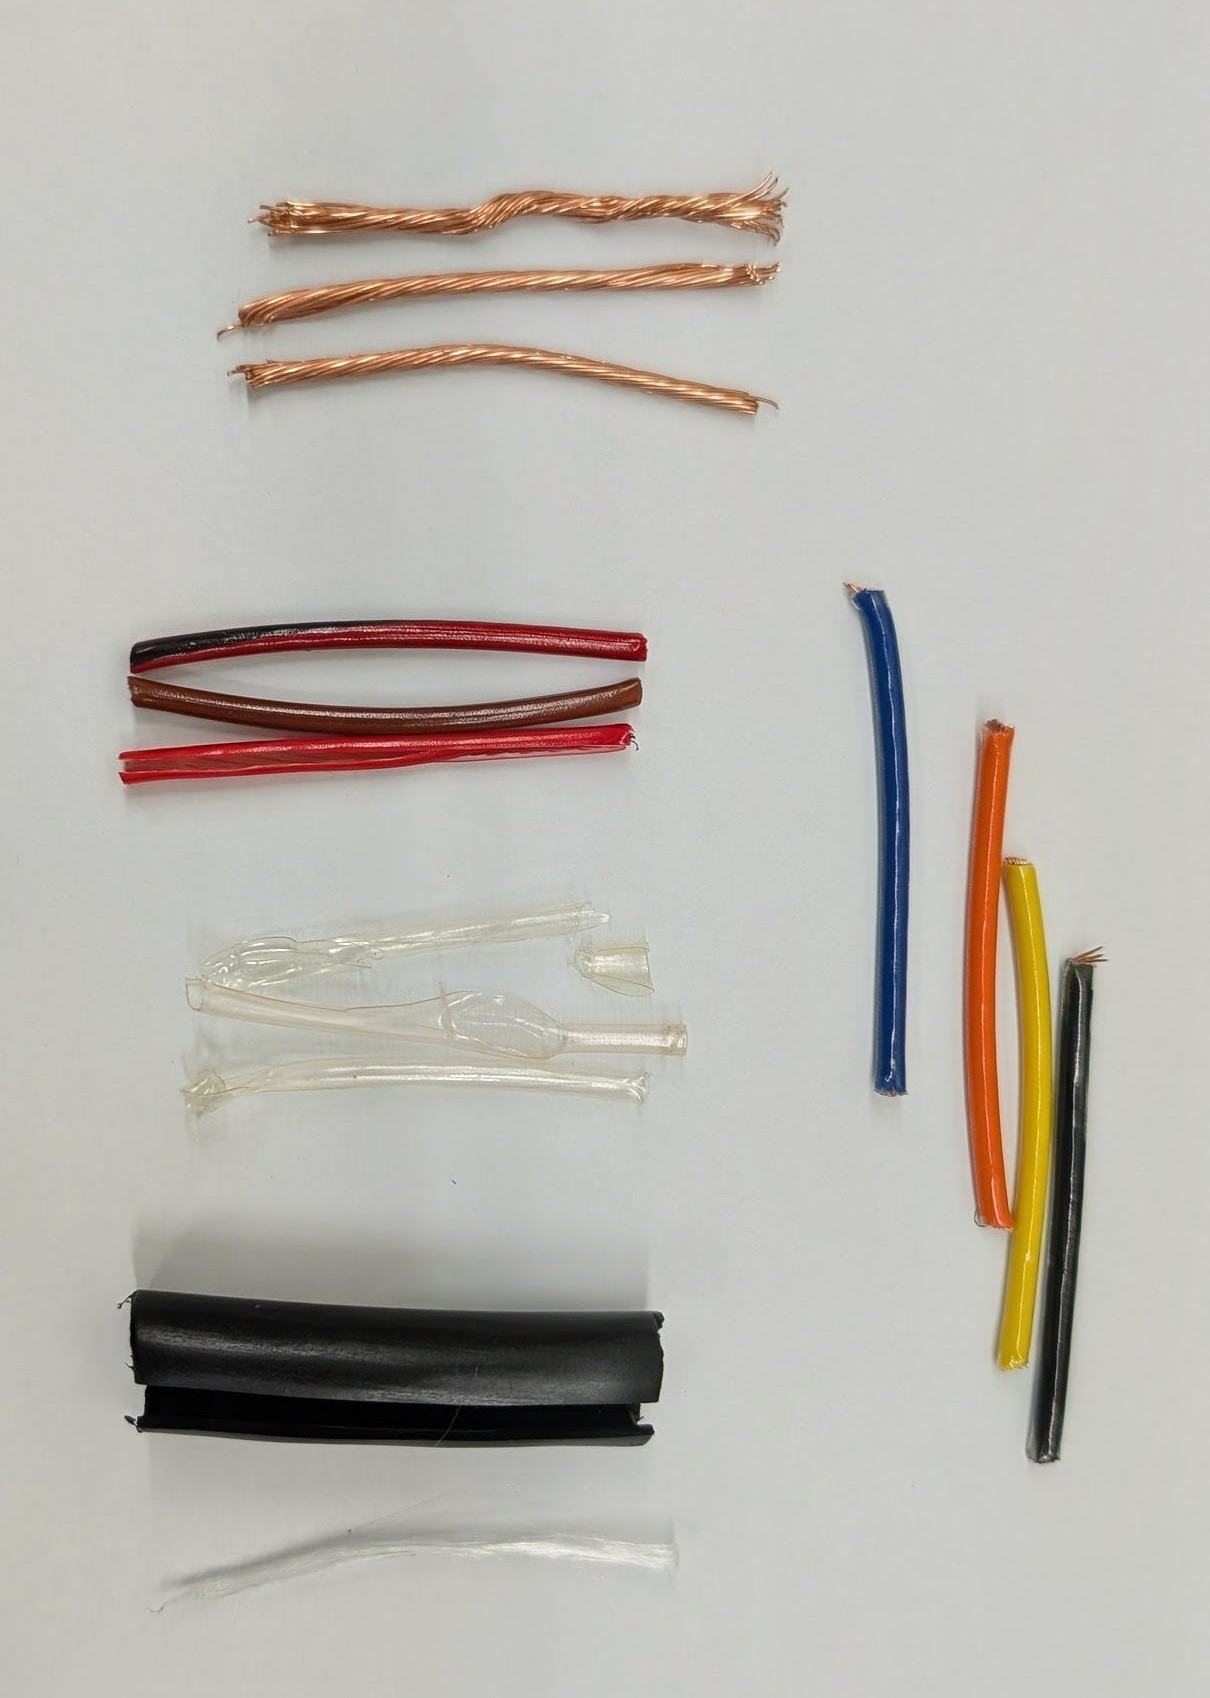
\includegraphics[width=0.7\linewidth, angle=-90]{../FIGURES/thermoplastic_components.jpg}
		\caption{Thermoplastic: 12-7C THHN/THWN }
		\label{fig:cable_components_tp}
	\end{subfigure}
	\hfill % Adds flexible space to push subfigures to edges
	\begin{subfigure}{0.49\textwidth}
		\centering
		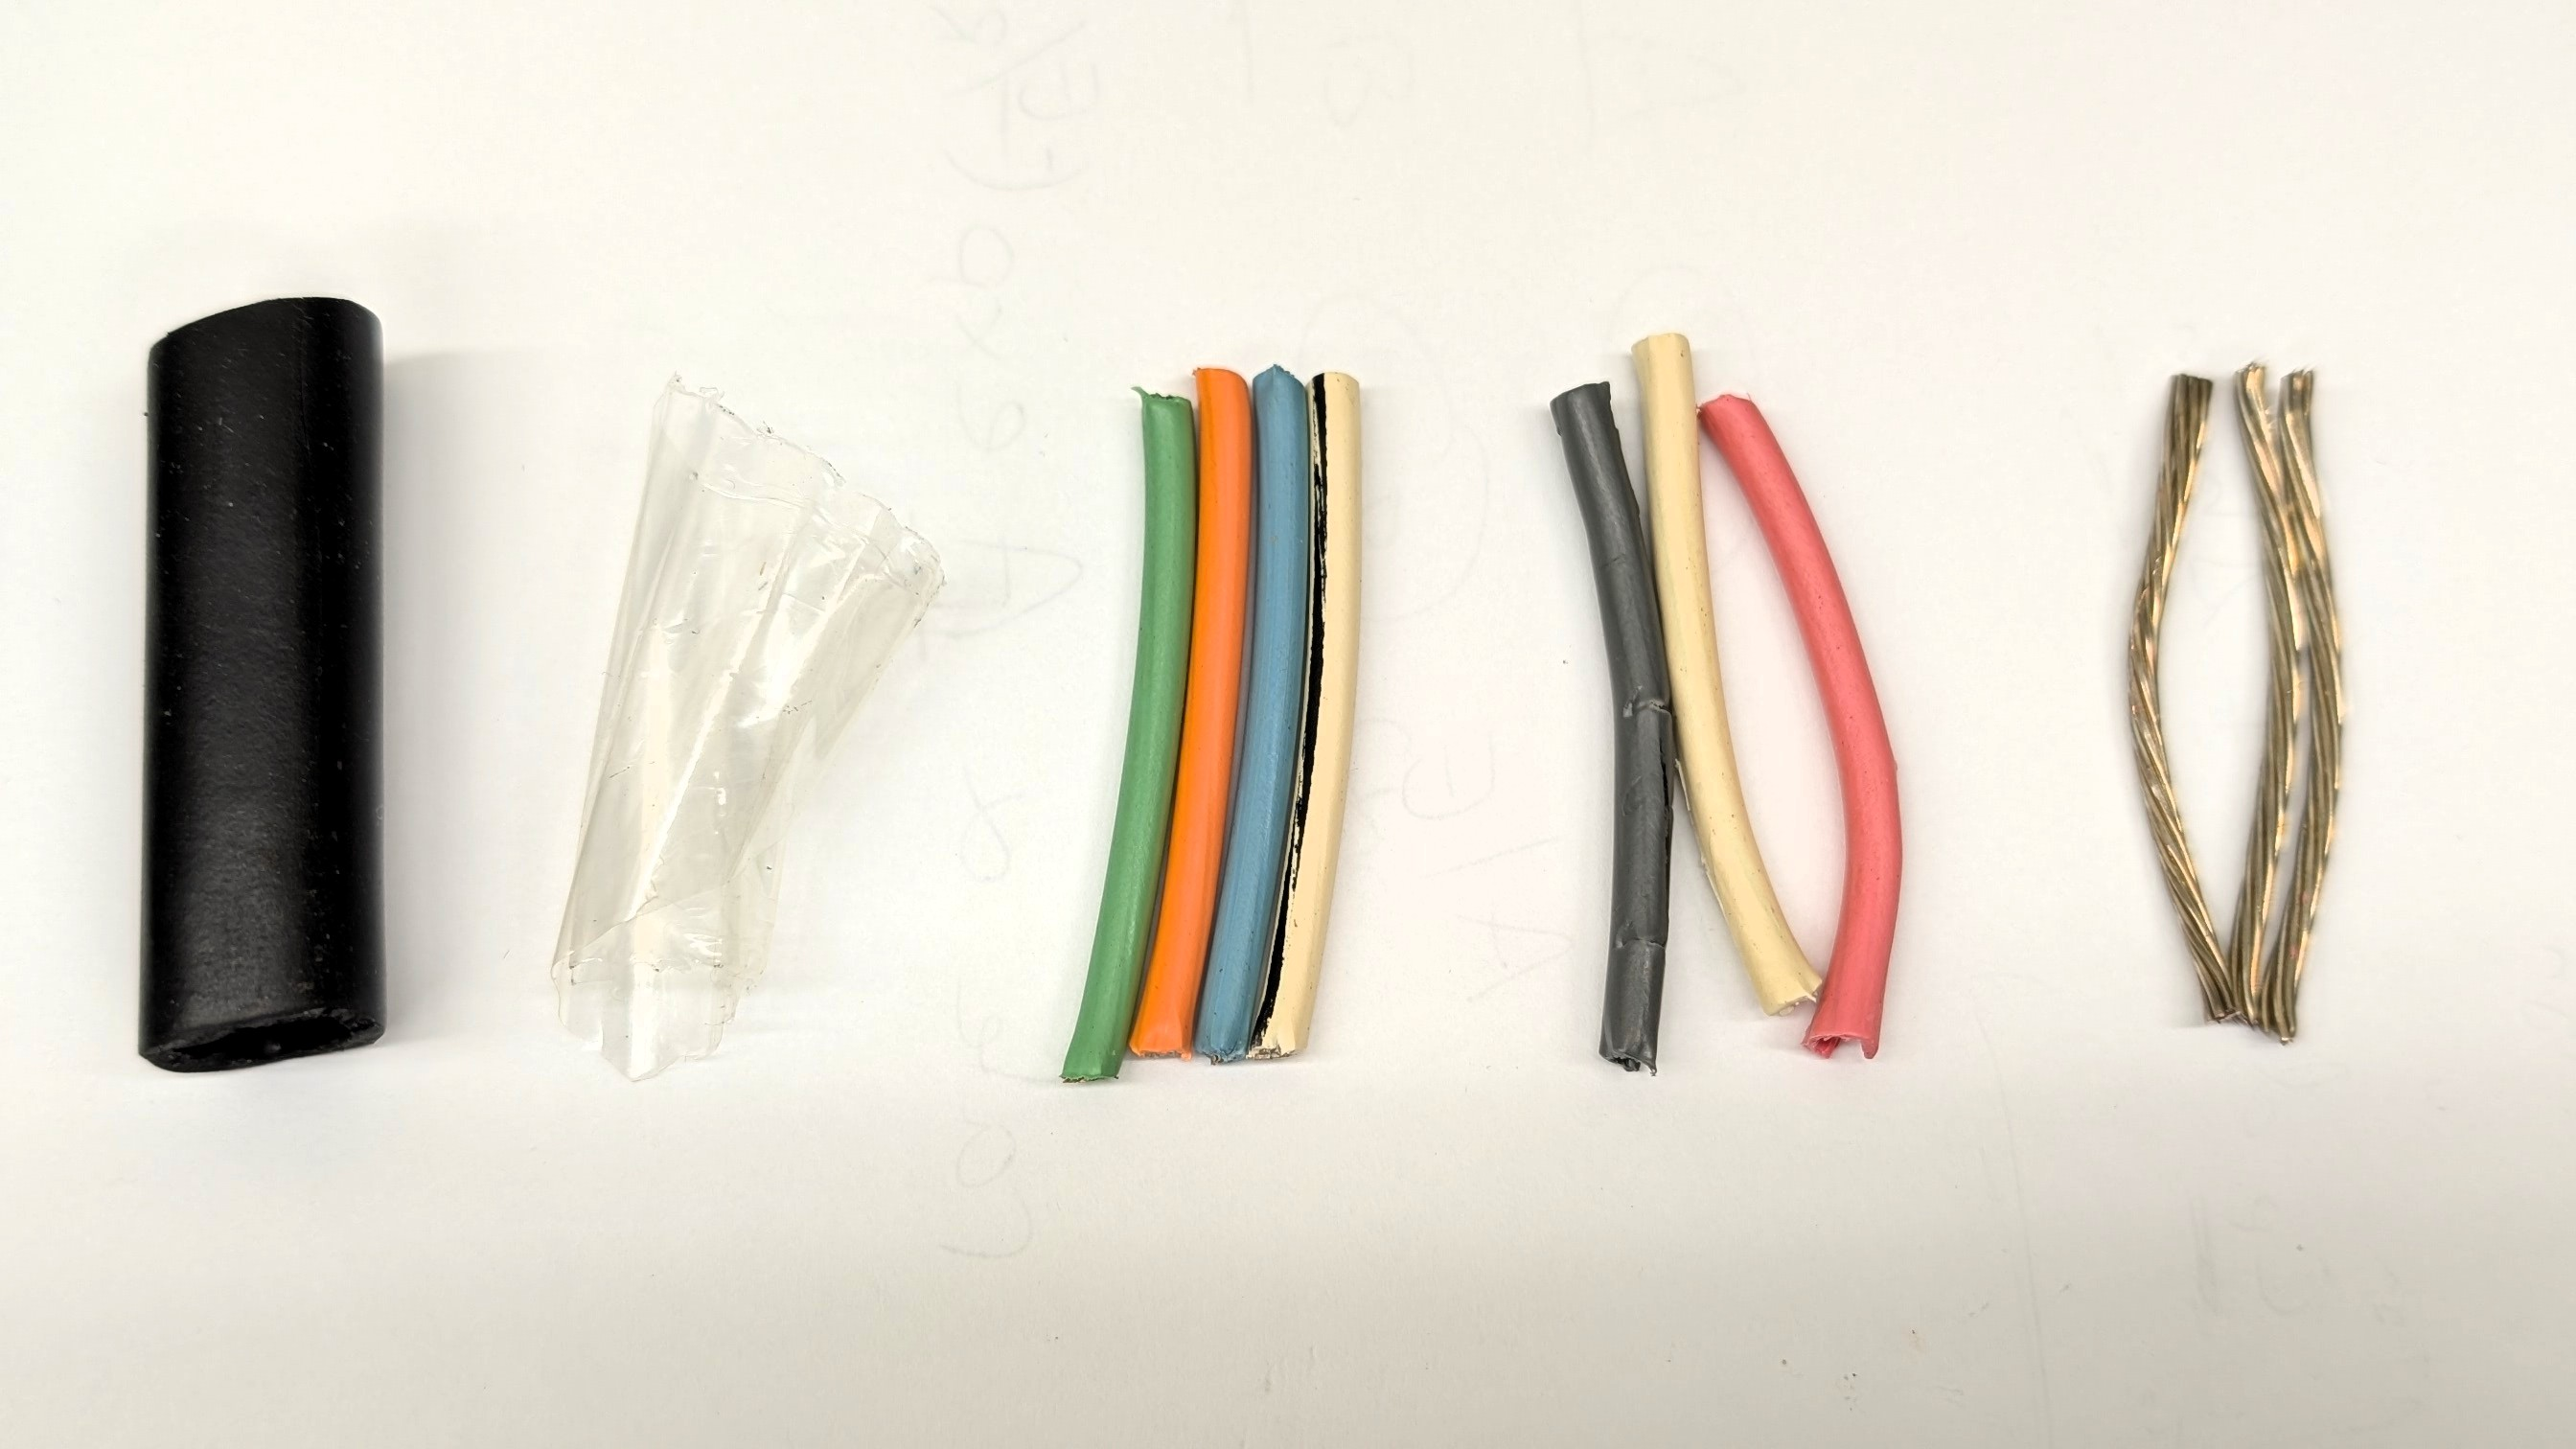
\includegraphics[width=\linewidth]{../FIGURES/thermoset_components.jpg}
		\caption{Thermoset: Firewall III}
		\label{fig:cable_components_ts}
	\end{subfigure}
	\caption{Representative images of the cables tested in this work, each separated into their main components: outer jacket, inner insulation, clear binder, and metal conductors.}
	\label{fig:cable_components}
\end{figure}

\begin{figure}[htbp]
	\centering
	\begin{subfigure}{0.49\textwidth}
		\centering
		\includegraphics[width=\linewidth]{../SCRIPT_FIGURES/Composition_total.pdf}
		\caption{Total cable mass.}
		\label{fig:cable_composition_total}
	\end{subfigure}
	\hfill % Adds flexible space to push subfigures to edges
	\begin{subfigure}{0.49\textwidth}
		\centering
		\includegraphics[width=\linewidth]{../SCRIPT_FIGURES/Composition_comb.pdf}
		\caption{Combustible components only.}
		\label{fig:cable_composition_comb}
	\end{subfigure}
	\caption{Relative mass fractions of cable components.}
	\label{fig:cable_composition}
\end{figure}


\begin{table}[h]
	\centering
	\begin{tabular}{rcc}
		\hline
		\textbf{Attribute} & \textbf{Thermoset} & \textbf{Thermoplastic} \\ \hline
		Manufacturer & Rockbestos & Global Cable \\ 
		Supplier & Marmon Industrial & Global Cable \\ 
		Trade Name & Firewall III & \#12-7C THHN/THWN \\
		Outer Jacket & Chlorosulfonated Polyethylene (CSPE)& poly(vinyl chloride) \\ 
		Clear coating & - & Nylon \\ 
		Insulation & Fire Retardant Cross-linked Polyethylene (XLPE) & poly(vinyl chloride) (PVC) \\ 
		Cable & Tin-Coated Copper & Fully-annealed stranded bare copper \\ \hline
	\end{tabular}
	\caption{Comparison of Thermoset and Thermoplastic Cables}
	\label{tab:cable_comparison}
\end{table}

\textbf{Coatings}

\subsection{Accelerated Aging Protocol}
Introduction to / Discussion on cable aging scaling approach.

Where / how to get kinetics?

Aging temperatures / durations (for kinetic calibration) + additional low temperature aging temperature for validation of scaling approach (under temperatures more similar to those expected in actual use)

\subsection{Material Property Tests**}
\subsubsection{Elongation at Break (EAB)}

Elongation at break tests were conducted in accordance with ASTM D***~\cite{}...
\subsubsection{Thermogravimetric Analysis (TGA)}

\begin{table}
	\caption[TGA Measurements]{TGA Measurements. **Comment on uncertainties}
	\label{tab:TGA}
	\begin{minipage}{\textwidth}
		\begin{tabular}{ccccc}
			\hline
			Matl.  & Heat of        & Solid Residue (at 700$^\circ$C)   & Onset              & Fire Growth             \\
			No.    & Combustion     & Yield            & Temperature        & Capacity (FGC)          \\
			& (kJ/g)         & (g/g)            & (°C)               & (J/(g~K))               \\ \hline
			3      &  13.9          & 0.29             & 315     & 80             \\
			\hline
		\end{tabular}
	\end{minipage}
\end{table}

\subsubsection{Microscale Combustion Calorimetry(MCC)}


\subsection{Response to Fire Tests}
\subsubsection{Cone Calorimeter}
\subsubsection{Direct Flame Impingement}


\subsection{Experimental Results}
\label{sec:results}

\subsection{Material Property Tests**}
\subsubsection{Elongation at Break (EAB)}

Elongation at break tests were conducted in accordance with ASTM D***~\cite{}...
\subsubsection{Thermogravimetric Analysis (TGA)}
\subsubsection{Microscale Combustion Calorimetry (MCC)}


%"MCC experiments were conducted in Summer, 2026. The material samples were subjected to a 80~mL/min nitrogen stream starting at a temperature of 75~°C, increasing linearly to 750~°C at a heating rate of 60~K/min. The pyrolyzed gases were combusted in an oxygen stream of 20~mL/min. Tests were repeated at least three times for each material. Nominal results are listed in Table~\ref{MCC}. The mass-weighted average heat of combustion of the materials tested is approximately 20~MJ/kg. Also reported in this table are the onset temperature and Fire Growth Capacity, FGC. The FGC is a physically-based parameter for early stage fire growth, derived from a simple burning model, that has been shown to rank commercial materials according to their behavior in bench scale flame and fire tests~\cite{lyon2021molecular}. The onset temperature is approximated by the temperature at which 5~\% of total heat release is measured, consistent with the definition of the FGC. Details of these calculations are provided elsewhere~\cite{DOT/FAA/TC-20/30, lyon2021molecular}.

\subsection{Response to Fire Tests}
\subsubsection{Cone Calorimeter}
\subsubsection{Direct Flame Impingement}


\begin{table}
	\caption[MCC Measurements]{MCC Measurements. The relative expanded uncertainty in the reported Heat of Combustion is approximately 6~\% of the measured value. The primary components of this uncertainty estimate include: (1) the relative expanded uncertainty of the heat released per unit mass of oxygen consumed, 5~\%~\cite{Huggett:1}; (2) the relative expanded uncertainty of the system flow rate, 2~\%; and (3) test repeatability, 2~\% or 2 standard deviations of replicate measurements. The relative expanded uncertainty in the solid residue yield is 2~\%, primarily due to stochastic variations in values measured in repeated tests.}
	\label{MCC}
	\begin{minipage}{\textwidth}
		\begin{tabular}{ccccc}
			\hline
			Matl.  & Heat of        & Solid Residue    & Onset              & Fire Growth             \\
			No.    & Combustion     & Yield            & Temperature        & Capacity (FGC)          \\
			& (kJ/g)         & (g/g)            & (°C)               & (J/(g~K))               \\ \hline
			3      &  13.9          & 0.29             & 300 & 80             \\
			\hline
		\end{tabular}
	\end{minipage}
\end{table}




\clearpage

\section{Conclusion}

Experiments were conducted to measure the heat release rate (HRR) and burning behavior of circuit breaker fires within closed steel enclosures. Of note:
\begin{itemize}
	\item Impact of aging on cable performance in reaction to fire tests
	\item Impact of aging on Apparent Decomposition (TGA/MCC)
	\item Impact of aging on EAB
	\item Comment on kinetic parameters: single set for all temperatures? 
	\item Comment(s) on accelerated aging - which kinetic parameters predict behavior best? Can TGA results be correlated to EAB?
\end{itemize}

General discussion on scaling/aging approach

\newpage

\section{Acknowledgment}

This research has been funded by the U.S. Nuclear Regulatory Commission, Office of Nuclear Regulatory Research, under the direction of **Names**.

Additional comments and advice were provided by **Other Names**.

Justin Pomerantz, Scott Bareham, and Ryan Greene assisted in conducting the EAB and Cone Calorimetry experiments. 




\clearpage
\section*{References}
\addcontentsline{toc}{section}{References}
\bibliographystyle{unsrt}
\bibliography{FDS_general}



\end{document}
